\begin{frame}{Context}{Collective Adaptive System (CAS) working group}
\begin{figure}
	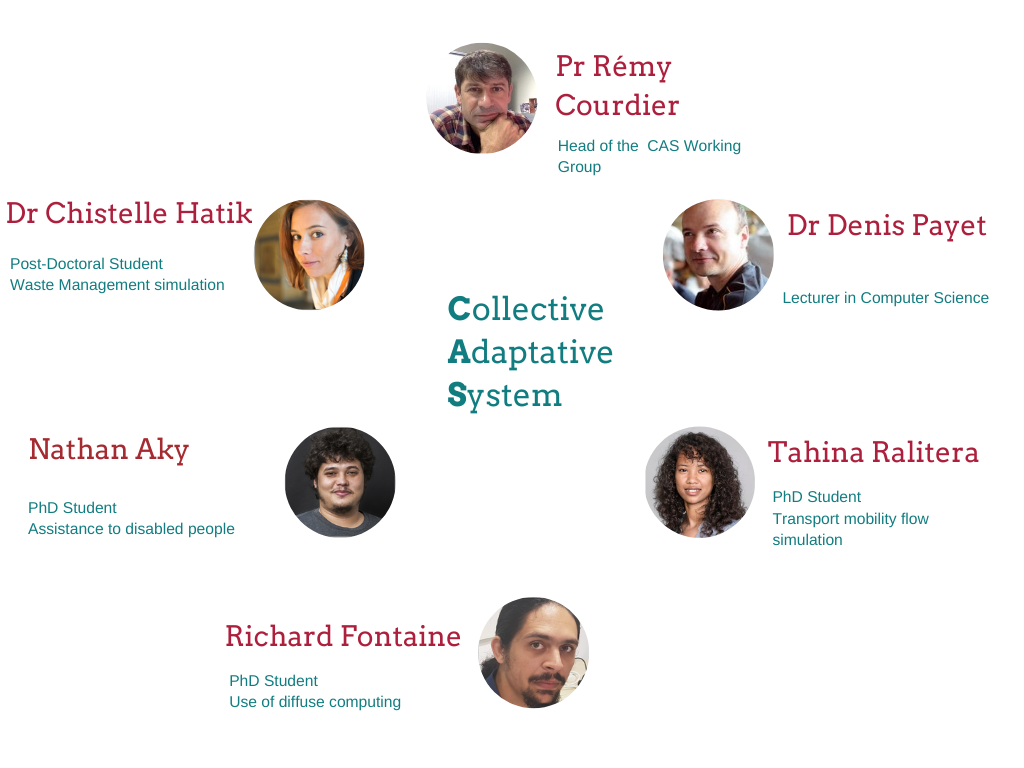
\includegraphics[width=.8\textwidth]{figures/SCA.png}
\end{figure}

\note{Cette thèse s’inscrit dans la continuité des travaux étudiés précédemment par le groupe de travail SCA du LIM qui se compose actuellement des personnes suivantes. Le groupe est spécialisé dans le paradigme des Systèmes Multi-Agents.

}
\end{frame}

%%%%%%%%%%%%%%%%%%%%%%%%%%%%%%%%%%%%%%%%%%%%%%%%%%%%

\begin{frame}{Context}{Collective Adaptive System (CAS) working group}
\begin{block}{Multi-Agent Systems}
\begin{itemize}
    \item Bottom-up approach
    \item The intelligence emerge from the agents interaction with the environment
\end{itemize}
\begin{figure}
	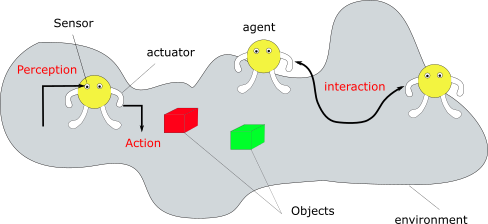
\includegraphics[width=.5\textwidth]{figures/SMA.png}
\end{figure}
\end{block}
\par Current team orientation: Towards hybrid approaches (simulation and real environment application)
\par However, \alert{my thesis focuses on multi-agent simulation (MAS)}

\note{Je vais donc commencer par définir les concepts de bases, ainsi que l'ensemble du jargon technique que j'utiliserai dans la suite de cette présentation et dans cette thèse. Un système multi-agent est un système composé d'un ensemble d'objets et d'agents situés dans un certain environnement et interagissant selon certaines relations. Un agent, à la différence d'un objet est une entité autonome et pro-active. Il est doté d'un ensemble de capteurs qui lui permet de percevoir son environnement. Cette perception lui permet de récupérer des informations. Il est également dotés d'un ensemble d'actionneurs qui lui permet d'agir sur ce dernier. Par exemple : il peut diffuser de l'information par le biais de l'environnement.
\par La modélisation à base de SMA est une approche ascendante. ie que  l'intelligence émerge alors de l'interaction entre les agents et l'environnement. 
\par Notre équipe s'est focalisé depuis plus de 20 ans sur la simulation multi-agents. Néanmoins notre politique actuelle s’oriente plus vers les approches de type hybrides. C’est-à-dire des approches qui combinent la simulation et l’application dans un environnement réel. Ainsi, bien que dans le cadre de cette thèse, je me concentre essentiellement sur la simulation, je prends tout de même en compte dans mes choix l’éventualité d’une future implémentation en milieu réel.

}
\end{frame}

%%%%%%%%%%%%%%%%%%%%%%%%%%%%%%%%%%%%%%%%%%%%%%%%%%

\begin{frame}{Context}{Multi-agent simulations of smart cities and smart islands}
\textbf{Sub-theme}: Application of multi-agent \alert{simulations} in the field of smart cities and smart islands. Example of London and Reunion Island cases. Collaboration with 
    \begin{figure}
	
\includegraphics[width=2cm]{assets/icl.png}
	\hspace{2cm}
	
\includegraphics[width=1cm]{assets/saintDenis.png}
    \end{figure}

\begin{block}{Smart City}
Using ICTs to solve the problems related to growing urbanization, the economic and environmental crisis that cities are currently facing and which put pressure on their structure and on the \alert{resources management}. 

\begin{itemize}
    \item The citizen participates proactively in the system 
    \item Bottom-up approach
    \item Participatory intelligence that emerges from interactions between the citizen and the system
\end{itemize}
\alert{MAS approach is a promising approach for smart city systems modeling}
\end{block}
\note{
Un des sous-thèmes que nous développons consiste en la simulation multi-agent appliquée aux villes intelligentes et aux îles intelligentes. Ma thèse s'inscrit dans ce contexte. Il s’agit d’un domaine en émergence dans notre équipe et sur lequel nous travaillons en collaboration avec des chercheurs de l'ICL et avec la mairie de Saint-Denis, La Réunion.
\par Comme il n'y a pas encore de standard permettant de définir ce qu'est une ville intelligente, nous aimerions clarifier notre vision de ce que c'est. Il s'agit bien évidemment d'une vision que nous partageons avec d'autres scientifiques travaillant dans le domaine. Le concept de smart city est considéré comme étant une solution technique qui consiste à utiliser les TIC pour résoudre les problèmes liés à l’urbanisation croissante, la crise économique et environnementale auxquelles les villes font actuellement face et qui mettent une pression sur leur structure et sur la gestion des ressources. Je met en évidence la gestion de ressources car il s'agit notamment de la problématique sur laquelle nous avons choisi de nous pencher dans notre exemple.
\par Par ailleurs, une particularité du concept qui le différencie de la ville classique est la place importante qu'occupe le citoyen au sein du système. En effet, le citoyen n'est pas vu comme un simple utilisateur qui subit le système, il y participe de manière proactive. 
\par L'intelligence dont il est sujet ici est alors une forme d'intelligence participative qui émerge des interactions entre les citoyens et le système. L'approche multi-agents est notamment une approche prometteuse permettant la modélisation de ce type de système.
}
    
\end{frame}

%%%%%%%%%%%%%%%%%%%%%%%%%%%%%%%%%%%%%%%%%%%%%%%%%

\begin{frame}{Context}{Multi-agent simulations of smart cities and smart islands}
\par \alert{Focus on smart mobility} : Multi-agent simulation of electric vehicles flow movement in a territory\footnote{https://www.flaticon.com/} 
\begin{figure}
	
\includegraphics[width=1.8cm]{figures/electric-car.png}
	\hspace{2cm}
	
\includegraphics[width=1.8cm]{figures/charging.png}
\end{figure}

\par \textbf{Objective}: optimise the time management of vehicle recharging with public charging points

\par \textbf{Problem}: Management of shared and limited resources in space and \alert{time}

\begin{itemize}
        \item \textbf{SkuadCityModel} : built upon the SimSKUAD platform, developed within our team
        \item \textbf{SmartCityModel} : built upon the Repast Simphony platform, developed by ICL, contribution of our team (2 scientific articles)
\end{itemize}

\note{
L’exemple sur lequel nous nous basons est celui du rechargement de véhicules électriques avec des bornes de recharge publiques dans l'objectif d'optimiser la gestion du temps de rechargement. Cet exemple rentre dans le contexte de la mobilité intelligente et illustre un problème plus général de gestion d'une ressource partagée et limitée dans l'espace et dans le temps que j'ai évoqué précédemment. Dans ce cadre nous décidons de nous concentrer plus sur l'aspect temporel pour des raisons que j'expliquerai dans le prochain diaporama.
\par Nous menons nos expérimentations et mettons en oeuvre nos solutions sur un modèle de simulation multi-agent de flux de déplacement de véhicules électriques sur un territoire appelé SkuadCityModel et une plateforme de simulation apelée SimSKUAD, que nous développons au sein même de notre équipe. Le modèle se base sur un modèle développé par les chercheurs de l’ICL appelé SmartCityModel, sur lequel nous avons également contribué et qui a fait l'objet de deux publications. Les problématiques abordées dans le cadre de cette thèse découlent des limites détectées lors de ces expérimentations.
}
    
\end{frame}

%%%%%%%%%%%%%%%%%%%%%%%%%%%%%%%%%%%%%%%%%%%%%%%
\begin{frame}{Problem}
\par \textbf{Problem}: Management of shared and limited resources in space and \alert{time}
\vspace{.5cm}
\par Focus on 2 aspect of time :
\begin{itemize}
    \item \textbf{The time representation} at the system level. Space, time and organization are the 3 important dimensions in the study of territorial systems \footnote{Rolland-May, C. (2000). Évaluation des territoires: concepts, modèle, méthodes. Hermès science publications.}. However, \alert{the temporal dimension (temporal dynamics) is often neglected}.
    \vspace{.3cm}
    \item \textbf{The temporal reasonning} at the agent level.  Taking into account past, present and future information in anticipatory reasoning is natural to humans. However, \alert{in most multi-agent simulations, agents do not consider information about the future (individual projects) in their reasoning}.
\end{itemize}
    
\note{
Notre étude du temps concerne deux aspects:
\begin{itemize}
    \item Au niveau du système, nous nous intéressons à la représentation du temps. Dans ce cadre nous constatons que dans les SMA, contrairement à une considération plus riche et plus complète de l'espace et des organisations, le temps y est généralement abordé uniquement sous un angle technique pour la synchronisation des entités du sytème. Nous pensons alors qu'il serait intéressant de compléter cette mécanique d'ordonnancement du temps par un support permettant l'échange d'informations sur la dimension temporelle, au même titre que la dimension spatiale et organisationnelle.
    \item Au niveau de l'agent, nous nous intéressons au raisonnement temporel. Plus particulièrement, sur la prise en compte des informations sur les 3 positions du temps linéaires : le passé (les souvenirs), le présent, le futur (les projets). Chez l'humain, la prise en compte des informations sur ces 3 dimensions du temps dans le processus de raisonnement anticipatif est naturelle. Cependant, à notre connaissance,la majorité des agents utilise dans leur modèle prédictif des informations positionnées uniquement sur le passé et sur le présent et ne prennent pas en compte le futur. Aucune information sur les projets individuels des agents n'est alors utilisé dans le raisonnement anticipatif malgré le fait que chaque agent dispose d'un planning qui devrait permettre de connaître, à l'avance, les activités que chacun prévoit d'effectuer. Cela est du à l'absence de visibilité sur la position futur du temps. Cette visibilité devrait justement être permis par le support de représentation du temps. Ce qui rejoint notre première problématique. 
\end{itemize}
}
\end{frame}

%%%%%%%%%%%%%%%%%%%%%%%%%%%%%%%%%%%%%%%%%%%%%%%%%%

\begin{frame}{Contributions}
\par \textbf{General objective}: consideration of the space, the organization and the time \alert{at the same level}.
\vspace{.5cm}
\par Contributions on 2 aspects:
\begin{itemize}
    \item \textbf{Time representation}: a medium that allows the exchange of temporal information on the same basis as spatial information and social information
    \vspace{.3cm}
    \item \textbf{Temporal reasoning}: enrichment of the information used at the level of the anticipative reasoning by taking into account the future. This is allowed by the medium that constitutes our first contribution
\end{itemize}
\note{
\par Notre objectif général est alors de considérer l'espace, le temps et les organisations au même titre. Cet objectif nous sert de base sur laquelle nous reposons nos choix. 
\par Afin de nous affranchir des limites citées précédemment, nous proposons 2 contribution
\begin{itemize}
    \item Au niveau de la représentation du temps : nous proposons de mettre en place un support permettant l’échange d’informations temporelles au même titre que les informations spatiales et sociales
    \item Au niveau du raisonnement temporel : nous proposons d'enrichir le raisonnement anticipatif par une prise en compte des informations temporelles positionnées sur le futur. Cela est permis par le support mis en place au niveau de la représentation du temps qui offre une visibilité sur la dimension future du temps.
\end{itemize}
Avant de rentrer plus en détails dans les contributions et pour une meilleure compréhension, je vais vous expliquer brièvement le fonctionnement général d’une simulation multi-agents avec un focus particulier sur la gestion du temps.
}
\end{frame}